
\chapter{Implementation: LSP server architecture}

The tool is integrated into IDEs via the Language server protocol. The goal is to give
users of the tool an overview of all clones as they appear in source-code.

The tool shows error-messages (diagnostics in LSP terms) which indicate which section of
code a clone covers, they also provide information about the matching clone and a
code-action to navigate to it.

The following user-stories shows how interaction with the LSP server works.

\begin{itemize}
	\item A programmer wants to see code clones for a file in their project, the
	      programmer opens the file in their IDE and is displayed diagnostics in the code
	      wherever there are detected clones. The matching code clones are not necessarily
	      in the same file.

	\item A programmer wants to see all code clones for the current project. The
	      programmer opens the IDEs diagnostic view and will see all code clones detected
	      as diagnostics there. The diagnostic will contain information like where the clone
	      exists, and where the matching clone(s) are.

	\item A programmer wants to jump to the corresponding match of a code clone in their
	      editor. The programmer moves their cursor to the diagnostic and will see a list of
	      the matching code clones. The programmer will select the wanted code clone which
	      will move the cursor to the file and location of the selected code clone.
          Alternatively, a code-action can be invoked to navigate, if the client does not
          implement the \verb|DiagnosticRelatedInformation| interface.

      \item A programmer wants to remove a set of clones by applying the
          ``extract-method'' refactoring. The programmer performs the necessary
          refactorings, saves the file and will get quick feedback whether the
          clones are now gone.
\end{itemize}

% TODO redo this figure
\begin{figure}
	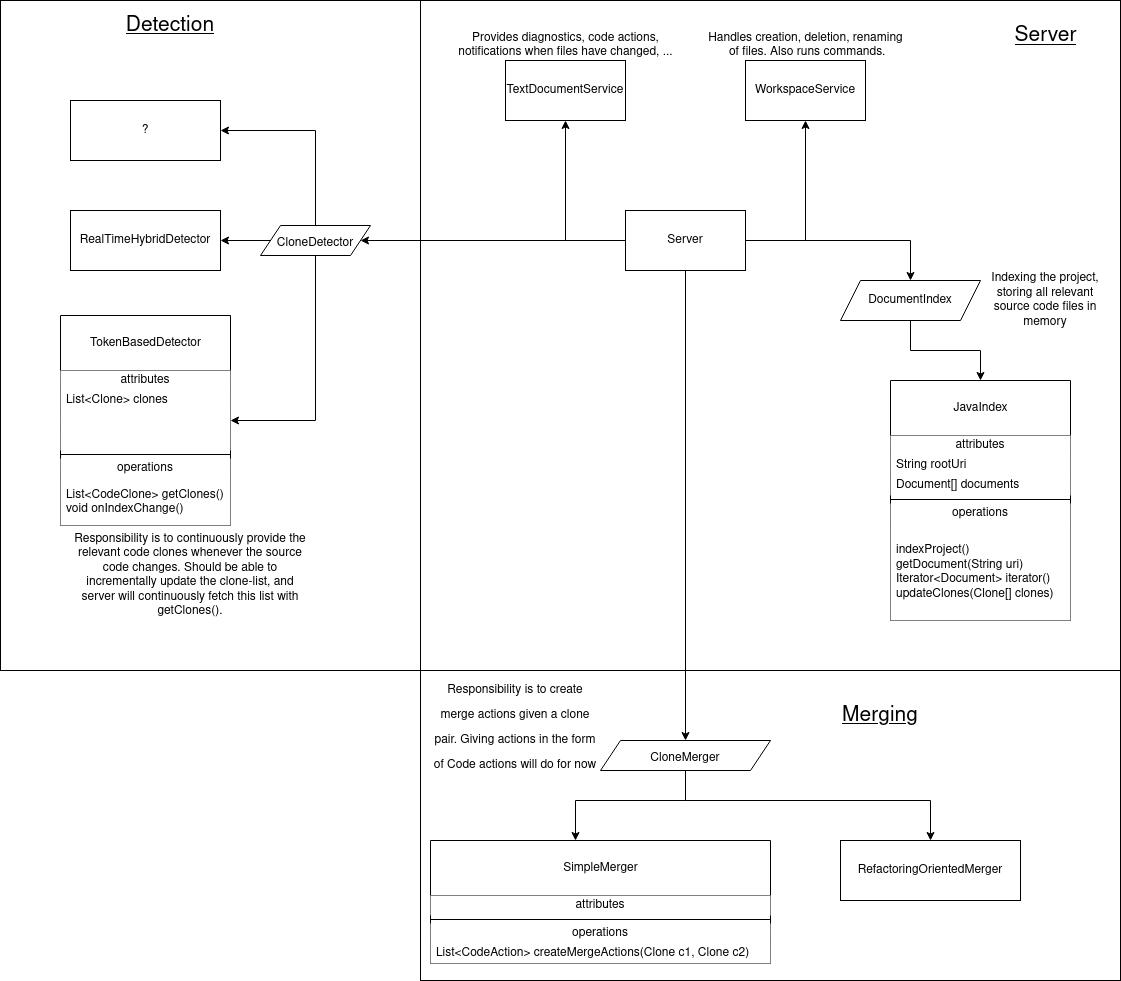
\includegraphics[width=\textwidth]{images/ToolArchitecture.png}
	\caption{Tool architecture}
	\label{fig:architecture}
\end{figure}

Figure \ref{fig:architecture} shows the architecture of the tool. The server communicates
with the IDE and delegates the work of managing clones to the detection engine and the
merge engine. The tool also stores an index of all source code files in the current project.

\section{Document index}

Upon starting, the LSP server requires indexing of the project for conducting analysis.
This involves creating an index and inserting the relevant documents. A document contains the
content of a file along with extra information such as the file's URI and information
about its clones.

There are two things to consider when determining which files should be inserted into the
index. First, we are considering only files of a specific file type, since the tool does
not allow analysis of multiple programming languages at the same time. Therefore, the
index should contain for example only \verb|*.java| files if Java is the language to
analyze. Secondly, all files of that file type might not be relevant to consider in the
analysis. This could for example be generated code, which likely contains a lot of
duplication, but is not practical or necessary to consider as duplicate code, since this
is not code which the programmer interact with directly. Therefore, the default behavior
is to consider only files of the correct file type, which are checked into Git. The tool
supports adding all files in a folder, or all files checked into Git.

When a document is first indexed by the server, the file contents is read from the disk.
However, as soon as the programmer opens this file in their IDE, the source of truth for
the files content is no longer on the disk, as the programmer is changing the file
continuously before writing to the disk. The LSP protocol defines multiple RPC
messages which the client sends to the server in order for the server to keep track of
which files are opened, and the state of the content of opened files.

Upon opening a file, the client will send a \verb|textDocument/didOpen| message to the
server, which contains the URI for the opened file. The index will at this point set the
flag \verb|isOpened| for the relevant document and stops reading its contents from disk.
Instead, updates to the file are obtained via the \verb|textDocument/didChange| message.
This message can provide either the entire content of the file each time the file changes,
or it can provide only the changes and the location of the change. Receiving only the
changes will be useful for this algorithm when the analysis incrementally reparses the
document.

\section{Displaying and interacting with clones}

\chapter{Implementation: Initial detection}


This section discusses the detection module of the tool. It consists of the detection
algorithm which takes the document index as input, and outputs a list of code clones. The
initial input to the algorithm will be the raw source code of each document in the index,
in text format.

The algorithm detects syntactical type-1 code clones, based on a token-threshold. Clones
detected are therefore snippets of source-code which has at least $N$ equal tokens, where
$N$ is a configurable parameter. There are also two types of clones which are filtered:

% TODO explain why where?
\begin{itemize}
    \item Clones which are completely contained within another larger clone.
    \item Clones which start in one fragment and ends in the next are cut off at the end
        of the first fragment.
\end{itemize}


In broad strokes, the algorithm first selects the relevant parts of source code to detect
code clones in (fragment selection), then transforms the selected fragments into a smaller
representation (fingerprinting). For the matching, an extended suffix array for the fingerprint
is constructed, where the LCP array is used to find matching instances of source-code.
Finally, clones are filtered and aggregated into clone classes before they are
source-mapped back to the original source-code locations, which the LSP server can display
as diagnostics.

\section{Fragment selection}

The first phase of the algorithm considers how to extract the relevant fragments of source
code which should be considered for detection. A fragment in this case is considered as a
section of abstract syntax, meaning that a particular type of node in the AST and the
tokens it encompasses should be extracted. Since the algorithm is language agnostic, it is
not feasible to have a single algorithm for fragment extraction or to define a separate
fragment extraction algorithm for every possible language. Therefore, the tool allows the
user to define a fragment query via tree-sitter queries\cite{treesitter}. Tree-sitter
queries are flexible queries to extract specific nodes or subtrees in an AST. For example,
in Java it would be natural to consider only methods. The tree-sitter query for selecting
only the method nodes in a Java programs AST would be:

\begin{equation}
    (\mathrm{method\_declaration\ } \text{@method})
\end{equation}

This tree-sitter query selects the node with type \verb|method_declaration| and
``captures'' it with the \verb|@method| name, for further processing by the program.
Readers interested in the details of the query system are referred to the tree-sitter
documentation\cite{treesitter}.

Implementing something similar for another parser/AST could be as simple as traversing
the tree until a node of a specific type is found, using the visitor pattern.

Using a tree-sitter query, the algorithm parses the program into an AST, queries the tree
for all the nodes which matches the query (taking care not to capture nodes which are
children of already captured nodes) and extracts all the tokens which the node covers.

\section{Fingerprinting}

\newsavebox{\firstlisting}
\begin{lrbox}{\firstlisting}
\begin{lstlisting}
public class Math() {
    public int multiplyByTwo(int param) {
        return param * 2;
    }

    public int addTwo(int param) {
        return param + 2;
    }
}
\end{lstlisting}
\end{lrbox}
\begin{figure}[htp]
	\begin{center}
        \subfloat[Source-code] {
            \usebox{\firstlisting}
        }
        \hspace{1cm}
        \subfloat[Fingerprint mapping] {
            \begin{tabular}{l | l}
                Token & Fingerprint \\
			    \hline
                public & 2 \\
                int & 3 \\
                multiplyByTwo & 4 \\
                ( & 5 \\
                param & 6 \\
                ) & 7 \\
                \{ & 8 \\
                return & 9 \\
                * & 10 \\
                2 & 11 \\
                ; & 12 \\
                \} & 13 \\
                addTwo & 14 \\
                + & 15 \\
            \end{tabular}
        }

        \vspace{0.5cm}
        \subfloat[Fingerprint, terminals highlighted] {
            [ 2, 3, 4, 5, 3, 6, 7, 8, 9, 6, 10, 11, \textbf{1}, 2, 3, 14, 5, 3, 6, 7, 8, 9, 6, 15, 11, \textbf{1}, \textbf{0} ]
        }
	\end{center}
	\caption{Example fingerprint of Java source-code}
	\label{fig:fingerprint}
\end{figure}

The next phase of the algorithm is to transform the extracted source code into a
representation which is less computationally heavy for the matching algorithm. The goal is
to reduce the total size of the input which needs to be processed by the matching
algorithm.

Since the algorithm that is used for matching is based on a suffix array, the
representation should be in a format similar to a string, which is the standard input to a
suffix array construction algorithm. However, it's not strictly necessary to use strings.
The essential property of the input array is that each element is comparable. Therefore,
we can use an array of integers instead, which is preferable, since there are often a lot
more unique integers available than unique characters in a programming language. The
algorithm will need to have a lot of unique elements in the representation because each
unique token value should be represented by one unique element, therefore integers are a
good choice.


The algorithm utilizes fingerprinting in order to reduce the size of the representation.
Fingerprinting is a technique which involves taking some part of the input and mapping it
to a smaller bit string, which uniquely identifiers that part. In this case, the algorithm
takes each token of the source-code, and maps it to an integers bit string. Each unique
token value (tokenized by tree-sitter) is mapped to unique integer values. Note that the
algorithm maps token values, not types. This ensures that tokens of different
variable-names and literals are not seen as equal. Figure \ref{fig:fingerprint} shows how
a sample Java program could theoretically be fingerprinted. The fingerprint mapping starts
its ``count'' at 2 to make space for some terminating characters. Each fragment is
terminated by a $1$ and the fingerprint is ultimately terminated by a $0$. Having these
values in the fingerprint will be useful for the matching algorithm where the suffix array
is constructed and utilized for detection.

The fingerprint of each fragment is stored in a list which the relevant document object
contains.



\section{Suffix array construction}

The next step is to input the fingerprint into a suffix array construction algorithm
(SACA), so that the suffix array can be used to find maximal repeats. All the fingerprints
which are stored in each document object are concatenated to be stored in a single integer
array (with terminators after each fragment), which the suffix array (SA), inverse suffix
array (ISA) and longest-common prefix array (LCP) is computed from.

We have utilized a straight-forward implementation of the ``Induced sorting
variable-length LMS-substrings'' algorithm~\cite{LinearTimeSuffixArraySAIS} which computes
a suffix array in linear time. The following section will give high-level overview of how
the algorithm works. 

The algorithm will be explained with a string input, as this is most common for suffix
arrays, and working with strings can be more clear to the reader when looking at suffixes.
The algorithm is still applicable to our fingerprint, since an array of integers will work
similarly to a string when given as input.

The ``Induced sorting variable-length LMS-substrings'' algorithm (often abbreviated SA-IS)
is an algorithm that works by divide and conquering the array and inducing how to sort the
bigger string from the smaller string, where the smaller string consists of the ``building
blocks'' of the bigger string. First, we will introduce some definitions and theorems used
for the algorithm. Input to the algorithm is a string $S$ with length $n$. Let
$\text{suffix}(S, i)$ be the suffix in S starting at position i.

\begin{definition}[L-type and S-type suffixes] A suffix starting at position $i$ in a
    string $S$ is considered to be L-type if it is lexicographically larger than the next
    suffix at position $i + 1$. Meaning that $\text{suffix}(S, i) > \text{suffix}(S,
    i+1)$. Conversely, a suffix is considered to be S-type if $\text{suffix}(S, i) <
    \text{suffix}(S, i+1)$. The sentinel suffix (\$) of $S$ is always S-type.
\end{definition}

Note that two suffixes cannot be lexicographically equal, therefore all cases are handled
by this definition. Determining the type of each suffix can be done in $O(n)$ by scanning
$S$ from right-to-left and observing the following properties. $\text{suffix}(S, i)$ is
L-type if $S[i] > S[i + 1]$. Similarly, $\text{suffix}(S, i)$ is S-type if $S[i] < S[i +
1]$. If $S[i] = S[i + 1]$, then $\text{suffix}(S, i)$ is the same value as
$\text{suffix}(S, i + 1)$. This is explained by the fact that if the first character of
the current suffix is not equal to first character of the next suffix, we already know the
type based on the first character. If the first character is equal however, we have
effectively reduced the case to the next suffix, since we are now comparing the second
character of the current suffix, with the next character of the second suffix. Since we
have already computed the type of that suffix, we can reuse the value. Figure
\ref{fig:sais-types} shows an algorithm which determines the type of each suffix in a
string in $O(n)$ time.

% TODO redo with pseudo-code
\begin{figure}
	\begin{center}
		\begin{lstlisting}
    private BitSet getSuffixTypes(String text) {
        boolean s_type = true;
        boolean l_type = false;
        int n = text.length;
        BitSet types = new BitSet(n + 1);
        
        if (n == 0) {
             return types;
        }

        types.set(n, s_type);
        types.set(n - 1, l_type);
        for (int i = n - 2; i >= 0; i--) {
            if (text[i] < text[i + 1]) {
                types.set(i, s_type);
            } else if (text[i] > text[i + 1]) {
                types.set(i, l_type);
            } else {
            types.set(i, types.get(i + 1))
            }
        }

    }
\end{lstlisting}
	\end{center}
	\caption{Algorithm to determine types of each suffix in a string}
	\label{fig:sais-types}
\end{figure}

\begin{algorithm}[htp]
  \SetAlgoLined\DontPrintSemicolon
    \algo{\SuffixTypes{S}}{
        $n \gets \text{S.length}$ \;
        $\text{Stype} \gets \text{true}$ \;
        $\text{Ltype} \gets \text{false}$ \;\;

        $\text{types} \gets \text{BitSet of size n}$ \;\;

        $\text{types.set}(n, \text{Stype})$ \;
        $\text{types.set}(n - 1, \text{Ltype})$ \;\;

        \For{$i \in (n - 2)..0$}{

            \uIf{$S[i] < S[i + 1]$}{
                $\text{types.set}(i, \text{Stype})$
            }
            \uElseIf{$S[i] > S[i + 1]$}{
                $\text{types.set}(i, \text{Ltype})$
            }
            \Else{
                $\text{types.set}(i, \text{types.get}(i + 1))$
            }
        }

        \Return types
    }

  \vspace{0.5cm}
  \caption{Compute suffix types of a string}
  \label{alg:suffixtypes}
\end{algorithm}


\begin{definition}[LMS character]

    An LMS (Left-most S-type) character in a string $S$ is a position $i$ in $S$ such that
    $S[i]$ is S-type and $S[i-1]$ is L-type. An LMS-suffix is a suffix in $S$ which begins
    with an LMS character. The final character of $S$ (the sentinel) is always S-type and
    the first character is always $L$ type

\end{definition}

\begin{definition}[LMS-substring]

    An LMS-substring in a string $S$ is a substring $S[i..j]$ in $S$ such that $i \neq j$,
    $S[i]$ and $[j]$ are LMS-characters and there are no other LMS-character between. The
    sentinel character is also an LMS-substring and is the only LMS-substring of length
    $\leq 3$

\end{definition}

LMS-substrings form "basic-blocks" in the string $S$. Each LMS-substring overlap on two
characters, and each substring should be monotonically decreasing, because of the type.
Using this notion, we can sort all LMS suffixes recursively with the following theorems:

\begin{theorem}
    Given sorted LMS-suffixes of $S$, the rest of the suffix array can be induced in linear
    time. 
\end{theorem}

\begin{theorem}
    There are at most $n / 2$ LMS-substrings in a string $S$ of length n.
\end{theorem}

The details of the theorems are left out, but the intuition of the second theorem will be
explained as it is the essential part of how the recursion allows us to build the suffix
array in linear time.

We can construct a smaller string $S_1$ by first sorting the LMS-substrings. Sorting
LMS-substrings can be done in linear time with a three-pass operation (details left out).
After sorting, each equal LMS-substring is given a unique increasing integer value. Two
LMS-substrings are considered equal if they are equal in terms of length, characters and
types. The smaller string is now built by mapping each LMS-substring in the original
ordering to its unique value, and forming a smaller string of it. of $S$ This smaller
string will be the reduced case which is used in the recursion. The string is at most $n /
2$ in size, meaning there will be at most $\log_2(n)$ recursive calls. The recursive call
will return the suffix array of the $S_1$. ~\cite{SuffixArrayConstruction} proves a
theorem which shows that sorting $S_1$ is equivalent to sorting the LMS suffixes of $S$.
Therefore, the suffix array of $S_1$ can be mapped to the LMS suffixes of $S$, which is a
subset of the SA of $S$. Now that we have

The base-case of the recursion will be when there is one LMS-substring, the sentinel
character. Intuitively, it is trivial to compute the suffix array of $S$ when there is
only one LMS-substring, since all suffixes except the sentinel are either in
lexicographically increasing or decreasing order. When the recursive call returns, the SA
of $S_1$ is used in another three-pass operation where the LMS suffixes guide the rest of
the suffixes to their correct location in SA.

There will be $O(\log_2(n))$ recursive call, where each recursive call takes $O(n)$ time,
with $n$ halving in each call. Therefore, the recurrence will have the complexity of:

\begin{gather*}
    T(n) =
\begin{cases}
    O(1) & \text{if } n = 1. \\
    T(n / 2) + O(n) & \text{if } n > 1.
\end{cases}
= O(n)
\end{gather*}

\subsubsection{Building ISA and LCP arrays}

Computing the ISA after constructing the SA is trivial. Since the ISA is simply the inverse
of SA, it can be constructed in linear time with a single loop as seen in Algorithm
\ref{alg:isa}

\begin{algorithm}[htp]
  \SetAlgoLined\DontPrintSemicolon
    \algo{\ISA{SA}}{
        $N \gets \text{SA.length}$ \\
        $\text{ISA} \gets int[N]$

        \For{$i \in 0..N$}{

            $\text{ISA}[\text{SA}[i]] \gets i$
        }

        \Return ISA
    }

  \vspace{0.5cm}
  \caption{Compute ISA from SA}
  \label{alg:isa}
\end{algorithm}


% TODO rewrite this shit
Computing the LCP in linear time is more complicated and requires some thought about which
order to insert LCP values. We will also add one extra restriction to the LCP values,
being that the LCP values cannot match past a $1$, which were the terminal value between
fragments. This restriction will be useful when we want to extract clones using the LCP.
The algorithm to compute the LCP is shown in Algorithm \ref{alg:lcp}. The intuition for
this algorithm is that if a suffix at position $i$ which has an LCP value $l$ describing
the common-prefix between it and some other suffix at position $j$, then the LCP value of
the suffix at position $i + 1$ is at least $l - 1$, since the suffix at $i + 1$ and $j +
1$ is the same suffix as the suffixes at position $i$ and $j$, with the first character
cut off. Therefore, they share at least $l - 1$ characters, and the algorithm can start
comparing the characters at that offset.

\begin{algorithm}[htp]
  \SetAlgoLined\DontPrintSemicolon
    \algo{\LCP{S, SA, ISA}}{
        $N \gets \text{SA.length}$

        $\text{LCP} \gets int[N]$

        $l \gets 0$

        \For{$i \in 0..N - 1$}{
            $r \gets \text{ISA}[i]$

            $\text{prevSuffix} \gets \text{SA}[r - 1]$

            \While{$S[i + l] = S[\text{prevSuffix} + l] \text{ and } S[i + l] \neq 1$}{
                $l \gets l + 1$
            }

            $\text{LCP}[r] \gets l$

            $l \gets \max{0, l - 1}$
        }

        \Return ISA
    }

  \vspace{0.5cm}
  \caption{Compute LCP from input string S, SA, and ISA}
  \label{alg:lcp}
\end{algorithm}


\section{Clone extraction}

With the extended suffix array structure, we can now consider which substrings (prefixes
of suffixes) we want to extract as potential code clones. In this phase the indices of the
fingerprint which we consider to be code clones are extracted, which will in the next
phase be used to map back to the original source code.

A solution is to extract every suffix which has an LCP value which is $\geq$ the token
threshold. This would be a single loop over $S$, using the inverse suffix array to find
the corresponding LCP value. This finds the clone indices, as shown in Algorithm
\ref{alg:simplecloneextraction}.

\begin{algorithm}[htp]
  \SetAlgoLined\DontPrintSemicolon
    \algo{\SimpleCloneExtraction{S, ISA, LCP}}{
        $n \gets \text{S.length}$ \;
        $\text{Clones} \gets List$ \;


        \For{$i \in 0..n - 1$}{
            \If{$\text{ISA}[i] = 0$}{
                \continue \;
            } \;

            \If{$LCP[ISA[i]] \geq \text{THRESHOLD}$}{
                $\text{clones.add}(i)$
            }
        }

        \Return clones
    }

  \vspace{0.5cm}
  \caption{Compute LCP from input string S, SA, and ISA}
  \label{alg:simplecloneextraction}
\end{algorithm}

However, this algorithm will return a lot of nested clones. This is because in a case
where there is a suffix with an LCP value of $100$, the next suffix will be of at least
$99$. Because of this, for any large code clone, there will be a lot of smaller clones
which are completely contained within it, but these clones are also likely to match with
another clone which is also contained within the larger clones match. In this way, the
contained clones are not very useful, and should not be considered. We extend our clone
extraction algorithm to account for this, by utilizing the following theorem:

\begin{theorem} The common prefix of a suffix at position $i$ is completely contained in
    the previous suffix at position $i - 1$ if the LCP value of the suffix at position $i
    - 1$ is greater than the LCP value of the suffix at position $i$. Meaning $LCP[ISA[i -
    1]] > LCP[ISA[i]]$
    
\end{theorem}


\section{Source-mapping}

\chapter{Implementation: Incremental detection}

\section{Updating the document index}

\section{Extracting edit operations}

\section{Dynamic suffix arrays}

\section{Storing old clones}


Remember to mention what we can afford to do and not.
